\section{System Design}
This section will first discuss how the system operates, by describing how the distributed game engine will operate.
After this, the fault-tolerance will be discussed and at last the scalability components of the system.

\subsection{System Operation}
The general setup of the DAS system consists of Master Servers, Helpers Server, Backup Servers, and Clients.
To initialize the game, one instance of the master server needs to be started. 
The master server will then contain the battlefield and a list of units playing on the battlefield.
The battlefield on this master server only contains a limited set of actions which can be performed.
The actual computation for these actions will not be be computed on the main server, but instead these will be computed on the helper servers.
Therefore for the game to function, it is important to also initialize at least one helper server. 
Every time a helper server is initiated, it also registers itself on the main server.
If a user starts the game on his computer, the clients then connects to main server requesting to join the game.
The master server then randomly selects a helper server from the list of his helpers servers.
The necessary details about the lucky helpers server is then returned to the client. 
The client then connects to this helper server and registers itself.
The client also requests the battlefield itself in order to be able to make the correct decisions. 
If everything works well: the user is ready to play!
When a user tries to perform an action, the action is sent to a helper server.
The helper server will then receive the request and, depending on the type of action, the helper with request the required information from the main server.
When this information is received, the helper performs the required computation of behalf of the player and sends the results to main server.
The server than send a message back to the client in order to inform him about the result of the action.

\begin{figure}[ht]
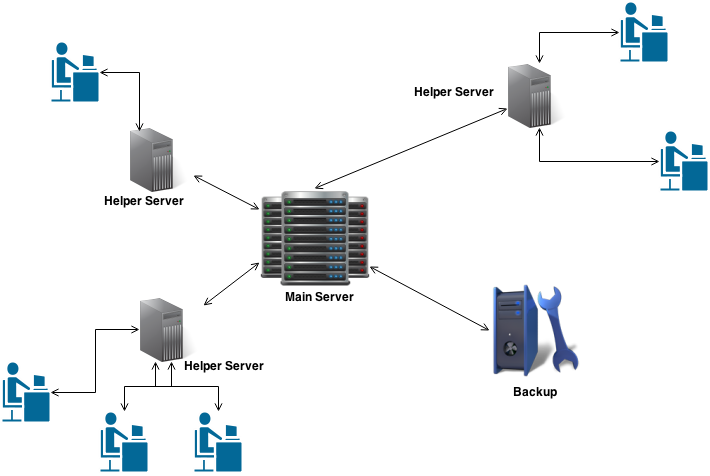
\includegraphics[scale=0.5]{DCS.png}
\end{figure}

\subsection{Fault Tolerance}
Every distributed system is prone to faults, and the Dragon Arena system is not an exception. 
First, lets look at the helper servers. As stated earlier, the clients connect to a helper server and register themselves there.
When a helper server goes down, the main server notices this and removes this helper from its known helpers.
If a client tries to query the helpers server when it wants to perform an action, it will detect that the helper server is down.
The client then asks the main server for a new helper server.
After the main server updates the client of his new helper, the client registers with the new helper and tries to execute its last action again.
The new helper receives the action request and continues working as usual.

It is also possible that the main server goes down. 
The main server was the one containing the data about the battlefield and its participants.
This is why it is necessary to have a backup server running.  
In order to recover when a main server crashes, the system does check-pointing periodically.
If during the periodic check, the main server detects that there has been changes to the battlefield, the main server sends the changes to the backup server.
The backup server then updates the knowledge of its backup battlefield and other relevant information.

If the main server goes down, it becomes impossible for the helper server to perform any action on the main server obviously.
If the helpers detect such a problem, they immediately try to send the request to the backup server and asks the backup server to perform the action requested on the battlefield.
The helpers also notify the backup, the failure of the main server and tell the main server that he needs to take over the tasks.
Whenever the backup server gets such a notification, it promotes itself to being the main server and takes all the responsibilities of a main server on itself.
The backup may be a few steps behind, because the backup is not made after each Unit action, but periodically. 
Updating the backup after each Unit action would cause too much overhead at the server.

\subsection{Scalability}
In order to support a large number of players on the battlefield, it is important for the system to be scalable.
As stated earlier, the helper servers are performing the computation for the main server.
It is possible to add as many helper server as possible which can be registered to the main server.
Clients may then connect to any of these available helper servers in order to play the game. One of the downsides of doing this is that; the more clients that are connected, the more helper servers you will need which might eventually flood the main server with requests. Another possible downside is; if one decides to spawn less helper servers, for example in order to prevent the previously described problem, one could put too many clients on a helper server, hence stressing the helper servers too much, which might make them unresponsive.

The main server on the other hand, is not scalable for distributing workload like the helper servers do. 
Instead, only a backup is created of the main server, which can be used if the main crashes.
Since the helper servers are the ones doing the computation, it is also not necessary for the main server to have multiple instances for distributing the workload.
 
